\section{Machine Learning}

After having sraped the articles for the documents \note{and sentiments?} a machine learning model was developed to predict stock price. \cref{fig:nn,fig:rnn} show the structure of a typical feed forward neural network and a recurrent neural network. Recurrent neural networks (RNNS), and others like RNNS, are particularly well suited to sie seues data

\cite{ko_lstm} show that an LSTM model, when trained on timeseries price data and sentiment data from news articles, can outperform a model trained on price data alone. Analysis of the literature suggests that SVM models, whilst the most popular \cite{al_literature_review} often underperformed in a financial setting, due to parameter optimisation being required \cite{al_literature_review,zhang_markov_model}

Talk about the adam optimiser \note{According to Kingma et al., 2014, the method is "computationally efficient, has little memory requirement, invariant to diagonal rescaling of gradients, and is well suited for problems that are large in terms of data/parameters". \cite{adam_keras_api_docs,adam_paper}}

\begin{figure*}[htbp]
    \centering
    \begin{minipage}{0.48\textwidth}
        \centering
        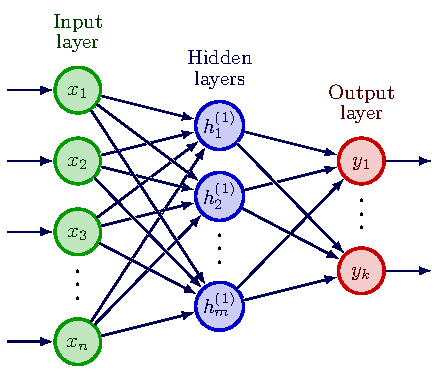
\includegraphics[width=\linewidth]{figures/nn}
        \caption{Typical "FeedForward" Neural Network Topology \cite{nn_diagram}}
        \label{fig:nn}
    \end{minipage}\hfill
    \begin{minipage}{0.48\textwidth}
        \centering
        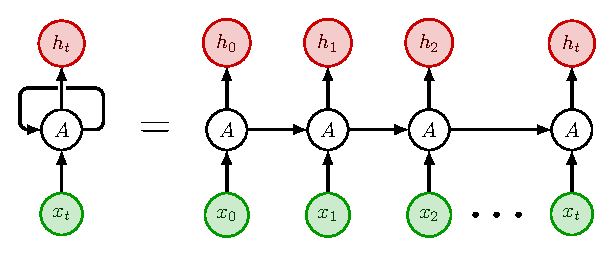
\includegraphics[width=\linewidth]{figures/rnn}
        \caption{Recurrent Neural Network Topology \cite{rnn_diagram}}
        \label{fig:rnn}
    \end{minipage}
\end{figure*}




\note{the
events extracted from the news are usually quite sparse, resulting in unreliable
and unsustainable predictive power \cite{zhang_markov_model} (bar for bar)}